\chapter{As cores e os espectros da luz}\label{ch:g8:colors-spectra}

Onde moram as cores? Na maçã, diz o bom senso --- o vermelho está
bem ali, na casca. E no entanto leve a maçã para um ginásio iluminado
de azul profundo e a maçã ``vermelha'' fica preta feito carvão. As
cores, acontece, são uma conversa a três entre a \omterm{def:g1:light-and-shadows:source}{luz}, o objeto e o
olho --- e ela começa com o fato mais estranho da óptica: a \omterm{def:g1:light-and-shadows:source}{luz}
branca não é branca.

\section{A luz branca desempacotada}

\begin{proposition}[A luz branca é uma mistura]\label{prop:g8:colors-spectra:mixture}
A \omterm{def:g1:light-and-shadows:source}{luz} ``branca'' comum --- a do Sol, a de uma lâmpada --- é uma
mistura de todas as cores ao mesmo tempo. Mandada por um prisma de
vidro, a mistura se desempacota: cada cor se entorta um pouquinho
diferente ao atravessar o vidro, e assim as cores se abrem em leque
numa faixa contínua do vermelho (o menos entortado) ao violeta (o
mais entortado). A faixa se chama \emph{espectro}\index{espectro}, e o
desempacotamento, \emph{dispersão}\index{dispersão}.
\end{proposition}

\begin{omfigure}
\begin{tikzpicture}[scale=0.85]
  \draw[-Stealth, very thick] (0.2,1.6) -- (3.2,1.6);
  \node[above, font=\small] at (1.5,1.75) {luz branca};
  \draw[thick, fill=blue!6] (3.4,0.4) -- (4.6,2.8) -- (5.8,0.4)
    -- cycle;
  \draw[red, very thick] (4.85,1.45) -- (9.6,1.15);
  \draw[orange, very thick] (4.85,1.45) -- (9.6,0.85);
  \draw[yellow!75!black, very thick] (4.85,1.45) -- (9.6,0.55);
  \draw[green!65!black, very thick] (4.85,1.45) -- (9.6,0.25);
  \draw[blue, very thick] (4.85,1.45) -- (9.6,-0.05);
  \draw[violet, very thick] (4.85,1.45) -- (9.6,-0.35);
  \node[right, font=\small] at (9.7,1.15) {vermelho: o menos entortado};
  \node[right, font=\small] at (9.7,-0.35) {violeta: o mais entortado};
  \node[below, font=\small] at (4.6,0.2) {prisma};
\end{tikzpicture}

{\small A \omterm{prop:g8:colors-spectra:mixture}{dispersão}: o prisma entorta cada cor da mistura branca com
a medida dela, e a mistura confessa --- um \omterm{prop:g8:colors-spectra:mixture}{espectro} do vermelho ao
violeta.}
\end{omfigure}

\begin{example}[Espectros sem laboratório]\label{ex:g8:colors-spectra:everyday}
A natureza e a gaveta de tralhas estão cheias de prismas. O arco-íris:
cada gotinha de chuva é um prisma-com-espelho em miniatura, e o arco
que cruza o céu é a \omterm{def:g1:light-and-shadows:source}{luz} do Sol dispersada por milhões de gotas ---
sempre na metade do céu \emph{oposta} ao Sol, motivo pelo qual os
caçadores de arco-íris ficam de costas para ele. A névoa fina da
mangueira do jardim conjura um sob encomenda. A face ranhurada de um
CD joga espectrinhos pelo teto; a borda chanfrada de um \omterm{def:g5:mirrors-reflection:reflection}{espelho}
listra a parede nas tardes de sol. A \omterm{def:g1:light-and-shadows:source}{luz} branca entrega a mistura
dela em todo lugar onde encontra estrutura fina ou vidro inclinado.
\end{example}

\begin{example}[Empacotando a mistura de volta]\label{ex:g8:colors-spectra:newtondisc}
O desempacotamento anda de trás para a frente. Pinte um disco com
setores de arco-íris e o gire depressa: o olho, lento demais para
acompanhar, recebe todas as cores praticamente de uma vez de cada
ponto --- e lê a mistura: um branco-cinza pálido e desbotado. O grande
físico que primeiro desempacotou a \omterm{def:g1:light-and-shadows:source}{luz} do Sol com um prisma girou
exatamente um disco desses para defender o empacotamento --- e o
lance mais ousado dele foi um segundo prisma, apanhando o \omterm{prop:g8:colors-spectra:mixture}{espectro} e
dobrando-o de volta num único \omterm{def:g6:light-propagation:ray}{feixe} branco: mistura provada nos dois
sentidos.
\end{example}

\begin{omfigure}
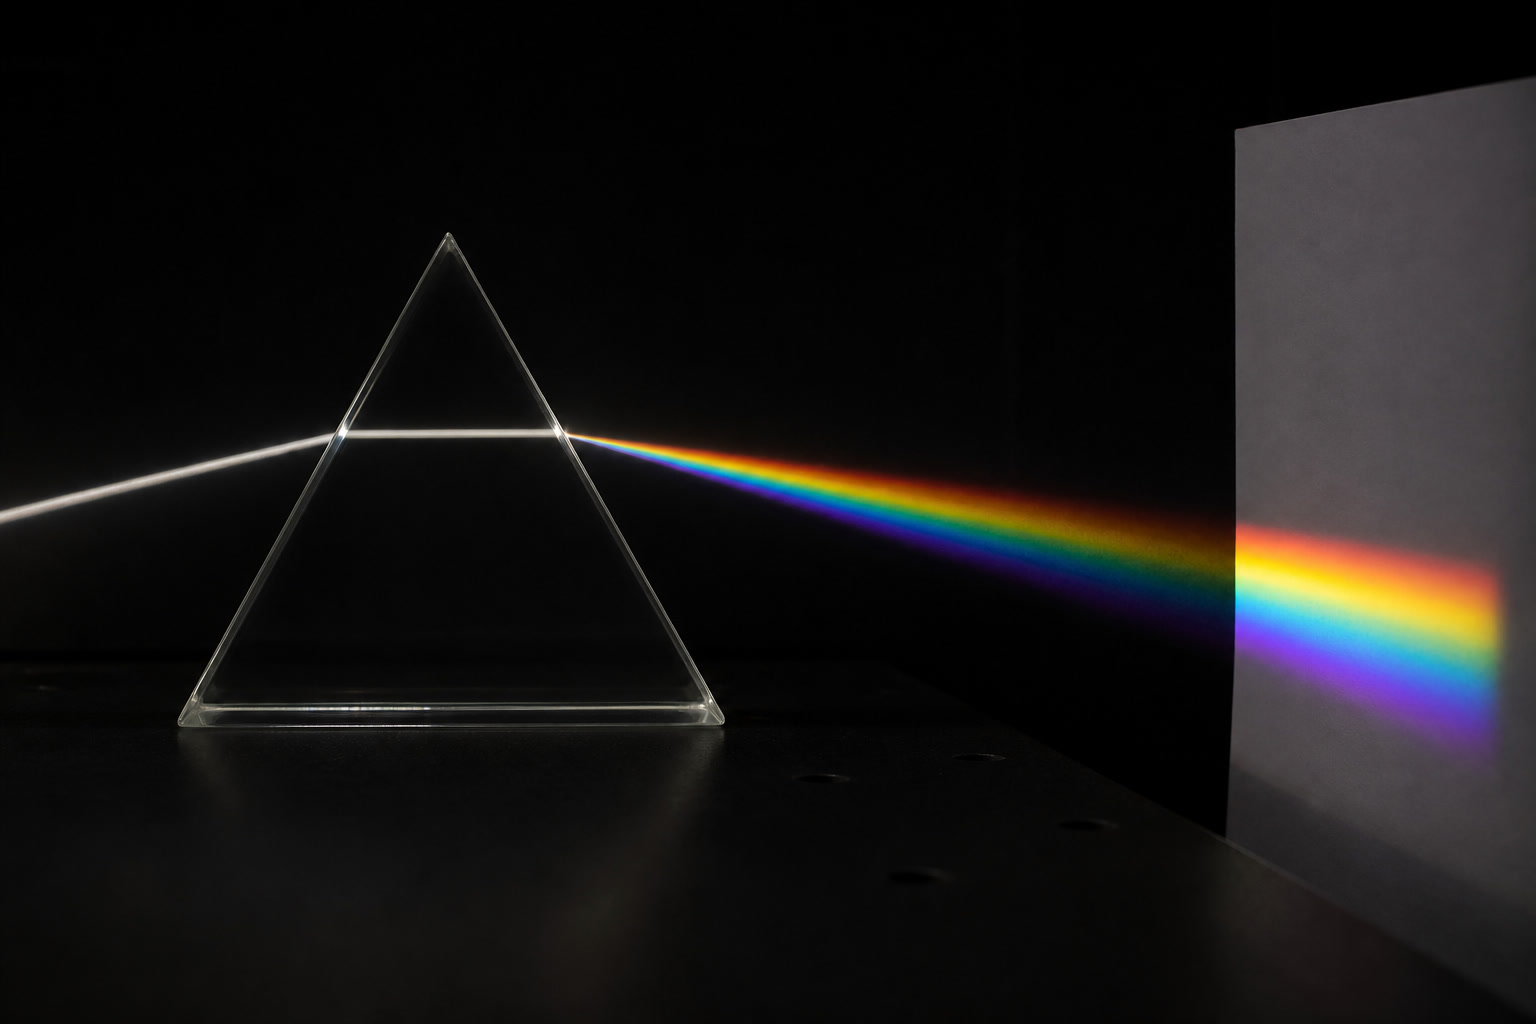
\includegraphics[width=0.55\linewidth]{images/book1/ai/g8-colors-prism.jpg}

{\small A \omterm{def:g1:light-and-shadows:source}{luz} branca desfeita por um prisma: as cores que ela sempre conteve se abrem em leque, o vermelho menos entortado, o violeta mais.}
\end{omfigure}

\section{Por que a maçã é vermelha}

\begin{proposition}[A cor de um objeto]\label{prop:g8:colors-spectra:objectcolor}
A cor de um objeto \omterm{def:g7:light-sources-propagation:coats}{opaco} é feita por subtração. Ao receber \omterm{def:g1:light-and-shadows:source}{luz}, o
objeto \emph{absorve} parte da mistura e difunde o resto --- e o
resto difundido é o que chega ao seu olho e dá nome à cor. Uma maçã
vermelha absorve quase todas as cores da \omterm{def:g1:light-and-shadows:source}{luz} branca e devolve
sobretudo o vermelho. Uma página branca devolve quase tudo; um casaco
preto devolve quase nada --- absorvendo a mistura inteira (e
esquentando na mesma medida, como os carros escuros testemunham no
verão). A cor não está \emph{na} casca: ela é a resposta da casca à
\omterm{def:g1:light-and-shadows:source}{luz} que lhe foi oferecida.
\end{proposition}

\begin{example}[O teste do ginásio]\label{ex:g8:colors-spectra:gym}
Agora, o ginásio iluminado de azul. A casca da maçã vermelha faz o
que sempre faz: absorve tudo menos o vermelho e fica pronta para
devolver vermelho --- mas o refletor azul não \emph{contém} vermelho
nenhum para ser devolvido. Nada difundido, nada recebido: a maçã se
mostra preta. A página branca sob a mesma \omterm{def:g1:light-and-shadows:source}{luz} devolve o que lhe é
dado: ela parece azul. Regra do teatro: um objeto só pode devolver as
cores que a \omterm{def:g1:light-and-shadows:source}{luz} trouxe --- mude a \omterm{def:g1:light-and-shadows:source}{luz} e você muda todos os figurinos
do salão.
\end{example}

\begin{omfigure}
\begin{tikzpicture}[scale=0.85]
  \fill[omExo, opacity=0.15] (0,0) rectangle (5.2,3.2);
  \draw[-Stealth, very thick] (0.4,2.5) -- (1.7,1.9);
  \node[above, font=\small] at (1.0,2.6) {luz branca};
  \draw[thick, fill=red!80] (2.4,1.4) circle (0.5);
  \draw[-Stealth, red, very thick] (3.0,1.7) -- (4.4,2.3);
  \node[right, font=\footnotesize, red] at (3.6,2.55)
    {vermelho devolvido};
  \node[below, font=\small] at (2.6,0.3) {parece vermelha};
  \begin{scope}[xshift=6.4cm]
    \fill[blue!20] (0,0) rectangle (5.2,3.2);
    \draw[-Stealth, very thick, blue] (0.4,2.5) -- (1.7,1.9);
    \node[above, font=\small, blue] at (1.0,2.6) {luz azul};
    \draw[thick, fill=black!85] (2.4,1.4) circle (0.5);
    \node[right, font=\footnotesize] at (3.1,1.9)
      {nada a devolver};
    \node[below, font=\small] at (2.6,0.3) {parece preta};
  \end{scope}
\end{tikzpicture}

{\small Uma maçã, duas \omterm{def:g1:light-and-shadows:source}{luzes}. A casca só devolve vermelho --- e sob
\omterm{def:g1:light-and-shadows:source}{luz} azul não chega vermelho nenhum para ser devolvido.}
\end{omfigure}

\begin{method}[Prever uma cor sob qualquer luz]\label{met:g8:colors-spectra:predict}
\begin{enumerate}
  \item liste o que a \omterm{def:g1:light-and-shadows:source}{luz} traz (branca: tudo; uma lâmpada colorida:
        sobretudo a cor dela);
  \item liste o que o objeto devolve sob \omterm{def:g1:light-and-shadows:source}{luz} branca --- a cor dele à
        \omterm{def:g1:light-and-shadows:source}{luz} do dia dá o nome;
  \item cruze as listas: o objeto difunde o que aparece nas duas;
  \item cruzamento vazio: o objeto se mostra preto.
\end{enumerate}
Um boné azul sob \omterm{def:g1:light-and-shadows:source}{luz} vermelha: devolve só azul, recebe só vermelho ---
cruzamento vazio: boné preto. Sob \omterm{def:g1:light-and-shadows:source}{luz} branca: a oferta completa
encontra a resposta azul --- boné azul.
\end{method}

\section{Construindo cores com luz}

\begin{example}[Três refletores fazem todas]\label{ex:g8:colors-spectra:additive}
Misturar \emph{\omterm{def:g1:light-and-shadows:source}{luzes}} soma. Superponha três refletores --- vermelho,
verde, azul: vermelho e verde juntos fazem amarelo; verde e azul, um
ciano turquesa; azul e vermelho, magenta; os três, branco. Com apenas
três primárias bem escolhidas, a mistura de \omterm{def:g1:light-and-shadows:source}{luzes} constrói
praticamente toda cor que o olho consegue nomear --- e é por isso que
três é o número mágico de toda tela luminosa.
\end{example}

\begin{example}[A tela no seu bolso]\label{ex:g8:colors-spectra:screen}
Examine uma área branca da tela de um celular ou de uma televisão com
uma lupa forte: branco nenhum em lugar algum --- só tirinhas
minúsculas vermelhas, verdes e azuis, todas em brasa. Toda cor que a
tela mostra são essas três lâmpadas em proporções dosadas; todo
``branco'' é o trio cantando a plenos pulmões, misturado pela
distância do seu olho. A caixa de tintas funciona ao contrário --- os
pigmentos absorvem, e misturá-los subtrai \omterm{def:g1:light-and-shadows:source}{luz} em vez de somá-la ---, e
é por isso que misturar todas as tintas dá uma escuridão barrenta
enquanto misturar todas as \omterm{def:g1:light-and-shadows:source}{luzes} dá branco; a história completa do
pintor pertence à aula de artes e à química.
\end{example}

\begin{remark}[O pôr do sol, pago integralmente]\label{rem:g8:colors-spectra:sunset}
A promessa do \omterm{def:g1:day-and-night:daynight}{pôr do sol} do ano passado vence hoje. O \omterm{def:g2:air-around-us:air}{ar} difunde a \omterm{def:g1:light-and-shadows:source}{luz}
do Sol --- mas não com imparcialidade: a ponta azul da mistura é
espalhada muito mais facilmente do que a vermelha. Olhe para longe do
Sol de dia e você vê a parcela roubada, reencaminhada pelo céu
inteiro: azul. No \omterm{def:g1:day-and-night:daynight}{pôr do sol}, a estrada rasante do \omterm{def:g6:light-propagation:ray}{feixe} direto pelo
\omterm{def:g2:air-around-us:air}{ar} é a mais longa e o roubo do azul é quase completo --- e o
sobrevivente que chega ao seu olho é o resto alaranjado e avermelhado,
com as nuvens cor-de-rosa apanhando os últimos espalhamentos. Céu
azul e \omterm{def:g1:day-and-night:daynight}{pôr do sol} vermelho são um roubo só, visto dos dois lados do
livro-caixa.
\end{remark}

\section{Exercícios}

\begin{exercise}[$\star$]\label{exo:g8:colors-spectra:1}
O que é um \omterm{prop:g8:colors-spectra:mixture}{espectro}, e o que é a \omterm{prop:g8:colors-spectra:mixture}{dispersão}? Qual cor se entorta menos
no prisma, e qual mais?
\end{exercise}

\begin{exercise}[$\star$]\label{exo:g8:colors-spectra:2}
Por que um caçador de arco-íris precisa ficar de costas para o Sol?
Quem faz o papel de prisma?
\end{exercise}

\begin{exercise}[$\star$]\label{exo:g8:colors-spectra:3}
Dê as duas demonstrações de que a \omterm{def:g1:light-and-shadows:source}{luz} branca é uma mistura --- uma
desempacotando, outra empacotando de volta.
\end{exercise}

\begin{exercise}[$\star$]\label{exo:g8:colors-spectra:4}
Na linguagem da subtração: por que a grama é verde? Por que a página
branca é branca e o quadro-negro é preto?
\end{exercise}

\begin{exercise}[$\star$]\label{exo:g8:colors-spectra:5}
Preveja com o método: um cachecol amarelo sob \omterm{def:g1:light-and-shadows:source}{luz} branca; sob \omterm{def:g1:light-and-shadows:source}{luz}
azul.
\end{exercise}

\begin{exercise}[$\star$]\label{exo:g8:colors-spectra:6}
Por que a maçã vermelha fica preta no ginásio azul --- e mesmo assim
o lenço branco ao lado dela fica azul?
\end{exercise}

\begin{exercise}[$\star$]\label{exo:g8:colors-spectra:7}
Diga as três primárias da mistura de \omterm{def:g1:light-and-shadows:source}{luzes} e os resultados de cada
superposição dois a dois --- e das três juntas.
\end{exercise}

\begin{exercise}[$\star$]\label{exo:g8:colors-spectra:8}
O que a lupa revela no ``branco'' de uma tela? Onde acontece a
mistura?
\end{exercise}

\begin{exercise}[$\star\star$]\label{exo:g8:colors-spectra:9}
Por que misturar todas as \emph{\omterm{def:g1:light-and-shadows:source}{luzes}} dá branco enquanto misturar
todas as \emph{tintas} dá uma escuridão barrenta? Uma frase para cada
lado do livro-caixa.
\end{exercise}

\begin{exercise}[$\star\star$]\label{exo:g8:colors-spectra:10}
Complete o livro-caixa do \omterm{def:g1:day-and-night:daynight}{pôr do sol}: o que o \omterm{def:g2:air-around-us:air}{ar} rouba com
preferência, quem recebe a mercadoria roubada e em que forma, e o que
sobrevive à estrada rasante mais longa --- e por que a \emph{\omterm{def:g2:moon-in-the-sky:moon}{Lua}
eclipsada} do ano passado brilha exatamente com esse sobrevivente.
\end{exercise}

\begin{exercise}[$\star\star$]\label{exo:g8:colors-spectra:11}
O provador de uma loja é iluminado com lâmpadas quentes avermelhadas,
``que favorecem o tom de pele''. Uma cliente compra uma jaqueta que
parecia de um marrom quente e profundo --- e a encontra verde-mate à
\omterm{def:g1:light-and-shadows:source}{luz} do dia. Reconstrua o engano com o método de previsão.
\end{exercise}

\begin{exercise}[$\star\star\star$]\label{exo:g8:colors-spectra:12}
Cenografia: uma projetista precisa de um estandarte com letras vivas
e legíveis sobre fundo preto sob a \omterm{def:g1:light-and-shadows:source}{luz} branca da plateia --- mas o
estandarte inteiro precisa sumir, uniformemente preto, letras e fundo
juntos, sob o banho vermelho profundo do finale. Escolha a cor das
letras e a cor do fundo (entre: branco, vermelho, verde, azul,
preto), justifique cada escolha com as regras da subtração e explique
por que letras \emph{brancas} --- a escolha tentadora --- trairiam o
finale.
\end{exercise}

\section{Problema: O teatro da luz}

\begin{problem}[{Problema de fim de semana --- ensaio geral sob
refletores coloridos; figurinos, filtros e uma cena sabotada; o exame
da projetista de iluminação}]\label{pb:g8:colors-spectra:1}
Ensaio geral: três refletores (vermelho, verde, azul) com dimmers, uma
arara de figurinos e um roteiro cheio de truques. O mapa de \omterm{def:g1:light-and-shadows:source}{luz} fica
com você.

\medskip\noindent\textbf{Parte I --- Exercícios de aquecimento.}
\begin{enumerate}
  \item Os três refletores no máximo: que \omterm{def:g1:light-and-shadows:source}{luz} banha o palco, e por
        quê?
  \item Vermelho e verde no máximo, azul apagado: dê o nome da \omterm{def:g1:light-and-shadows:source}{luz} do
        palco.
  \item Sob essa mistura vermelho-verde, preveja a aparência de: uma
        camisa branca; uma faixa azul; um vestido amarelo.
  \item O ciclorama branco do fundo sob o azul sozinho --- e o motivo
        de um fundo de palco ser sempre pano branco.
\end{enumerate}

\medskip\noindent\textbf{Parte II --- Clínica de figurinos.}
\begin{enumerate}[resume]
  \item O casaco do vilão precisa parecer preto na cena um (banho
        vermelho) e de um verde rico na cena dois (\omterm{def:g1:light-and-shadows:source}{luz} branca). Que
        cor de casaco à \omterm{def:g1:light-and-shadows:source}{luz} do dia serve, e por quê?
  \item O manto do fantasma precisa continuar parecendo branco em
        \emph{toda} iluminação. Que cor de manto, e o que ele vai
        mostrar de fato sob cada refletor sozinho?
  \item O cachecol vermelho de um ator precisa ``sangrar até sumir''
        --- indistinguível da cortina preta --- num certo momento.
        Que refletores podem ficar acesos para o truque, e por que
        ele fracassa no instante em que o refletor vermelho se junta
        a eles?
  \item As letras douradas do programa ficaram esplêndidas ao
        meio-dia mas barrentas sob a marcação noturna carregada de
        azul. Explique, tratando o dourado como um amarelo quente.
\end{enumerate}

\medskip\noindent\textbf{Parte III --- A sabotagem.}
Cena de abertura: o arco de arco-íris do cenário (listras pintadas:
vermelho, laranja, amarelo, verde, azul, violeta) sob \omterm{def:g1:light-and-shadows:source}{luz} branca
plena.
\begin{enumerate}[resume]
  \item Um brincalhão troca a marcação branca por vermelho puro.
        Listra por listra, o que a plateia vê agora?
  \item A diretora, improvisando, pede os refletores vermelho
        \emph{e} azul juntos. Que listras ressuscitam, e o que o
        banho amagentado faz com a listra verde?
  \item O contrarregra pergunta por que o arco não pode simplesmente
        ser ``iluminado de volta ao normal'' com um único refletor
        verde muito forte. Responda com a única \omterm{def:g1:light-and-shadows:source}{luz} que mostra as
        seis listras.
  \item Escreva a resposta de exame da projetista: as duas leis do
        teatro da \omterm{def:g1:light-and-shadows:source}{luz} --- uma sobre o que as \omterm{def:g1:light-and-shadows:source}{luzes} fazem quando
        misturadas, outra sobre o que os objetos fazem com o que lhes
        é dado --- cada uma em uma frase.
\end{enumerate}
\end{problem}
